\chapter{De opsplitsing van het leven}\label{ch:g12:diversification-of-life}

Broodtarwe heeft 42 \omterm{def:g10:universal-dna:information}{chromosomen}, in zes sets van zeven: zij is de som van
drie wilde grassen die twee keer zijn gekruist, op de akkers van de
eerste boeren. Een python heeft driehonderd wervels en een muis dertig,
en toch bouwen zij hun ruggengraat met dezelfde \omterm{def:g10:universal-dna:gene}{genen}. Een korstmos op een
rots bestaat uit twee organismen, een schimmel en een alg, die al zo lang
als één leven dat geen van beide nog alleen te vinden is. En een jonge
chimpansee leert noten met een steen kraken door naar zijn moeder te
kijken, in een bos waar de chimpansees honderd kilometer verderop dat
nooit hebben geleerd. \omterm{def:g11:mutations:mutation}{Mutatie} en het schudden van het vorige hoofdstuk
zijn niet de enige manieren waarop levende wezens verschillend worden;
dit hoofdstuk zet de andere op een rij.

\section{Meer dan mutatie}

\begin{proposition}[Bronnen van opsplitsing]\label{prop:g12:diversification-of-life:sources}
Puntmutaties en het geslachtelijke schudden scheppen nieuwe \omterm{def:g10:universal-dna:gene}{allelen} en
nieuwe combinaties daarvan. Daarbuiten is de verscheidenheid van levende
wezens voortgebracht door processen die het genoom op grotere schaal
veranderen --- \omterm{def:g10:universal-dna:gene}{genen} verdubbelen, \omterm{def:g10:universal-dna:gene}{genen} uit andere \omterm{def:g10:biodiversity-scales:species}{soorten} binnenhalen,
hele sets \omterm{def:g10:universal-dna:information}{chromosomen} toevoegen --- door veranderingen in de manier
waarop bestaande \omterm{def:g10:universal-dna:gene}{genen} tijdens de ontwikkeling worden gebruikt, door
verbonden tussen \omterm{def:g10:biodiversity-scales:species}{soorten}, en, bij dieren, door gedrag dat zonder enig \omterm{def:g10:universal-dna:gene}{gen}
wordt doorgegeven.
\end{proposition}
\admitted

\section{Nieuwe genen uit oude}

\begin{proposition}[Genverdubbeling en uiteengroeien]\label{prop:g12:diversification-of-life:duplication}
Een ongelijke \omterm{prop:g12:meiosis-genetic-shuffling:crossingover}{crossing-over} (\cref{ch:g12:meiosis-genetic-shuffling}) of
een kopieerfout kan een \omterm{def:g11:cell-cycle-mitosis:chromosome}{chromosoom} met twee kopieën van een \omterm{def:g10:universal-dna:gene}{gen}
achterlaten. De ene kopie blijft haar oorspronkelijke werk doen; de
andere, van die verplichting verlost, hoopt \omterm{def:g11:mutations:mutation}{mutaties} op en kan een nieuwe
functie krijgen --- of verloren gaan. Over evolutionaire tijd herhaald
levert dat \emph{genfamilies}\index{genfamilie} op: groepen verwante \omterm{def:g10:universal-dna:gene}{genen}
die van één voorouder afstammen en waarvan de mate van gelijkenis de
volgorde van de verdubbelingen vastlegt.
\end{proposition}
\begin{proof}[Bewijsmateriaal]
De drie \omterm{def:g11:the-eye:photoreceptors}{opsines} en het rodopsine uit \cref{ch:g11:the-eye} vormen zo'n
familie; de globines zijn er nog een: de verscheidene \omterm{def:g10:universal-dna:gene}{genen} voor de
ketens van hemoglobine --- één gebruikt in het embryo, één in de foetus,
twee bij de volwassene --- en het \omterm{def:g10:universal-dna:gene}{gen} van myoglobine, de zuurstofvoorraad
van de spier, liggen in trosjes op twee \omterm{def:g10:universal-dna:information}{chromosomen}, zijn voor 40\% tot
80\% gelijk in volgorde, en hun boom komt overeen met de volgorde waarin
de groepen \omterm{def:g10:common-ancestry:bodyplan}{gewervelden} verschenen. Genomen dragen honderden van zulke
families, en een aanzienlijk deel van elk genoom bestaat uit verdubbelde
stukken.
\end{proof}

\begin{omfigure}
\begin{tikzpicture}[font=\small, line cap=round, >=Stealth]
  \tikzset{g/.style={draw, fill=omDef!30, minimum height=0.45cm, minimum width=1.2cm, inner sep=1pt, font=\scriptsize}}
  % step 1: one gene
  \draw[thick] (0,3) -- (4,3); \node[g] at (2,3) {globine};
  \node[anchor=east] at (-0.2,3) {voorouderlijk gen};
  \draw[->, thick] (2,2.65) -- (2,2.15) node[midway, right] {verdubbeling};
  % step 2: two identical copies
  \draw[thick] (0,1.8) -- (5.4,1.8); \node[g] at (1.6,1.8) {globine}; \node[g] at (3.4,1.8) {globine};
  \node[anchor=east] at (-0.2,1.8) {twee kopieën};
  \draw[->, thick] (2.5,1.45) -- (2.5,0.95) node[midway, right] {in elk hopen zich mutaties op};
  % step 3: diverged
  \draw[thick] (0,0.6) -- (5.4,0.6); \node[g, fill=omThm!30] at (1.6,0.6) {$\alpha$-globine}; \node[g, fill=omMeth!30] at (3.4,0.6) {$\beta$-globine};
  \node[anchor=east] at (-0.2,0.6) {twee genen};
  \draw[->, thick] (2.5,0.25) -- (2.5,-0.25) node[midway, right] {verdere verdubbelingen};
  \draw[thick] (0,-0.6) -- (7.6,-0.6);
  \node[g, fill=omThm!30] at (1.0,-0.6) {$\zeta$}; \node[g, fill=omThm!30] at (2.4,-0.6) {$\alpha$};
  \node[g, fill=omMeth!30] at (4.2,-0.6) {$\varepsilon$}; \node[g, fill=omMeth!30] at (5.5,-0.6) {$\gamma$}; \node[g, fill=omMeth!30] at (6.8,-0.6) {$\beta$};
  \node[anchor=east] at (-0.2,-0.6) {een genfamilie};
  \node[anchor=west, align=left, font=\scriptsize] at (7.9,-0.6) {ketens van embryo,\\ foetus en volwassene};
\end{tikzpicture}

{\small Hoe een \omterm{prop:g12:diversification-of-life:duplication}{genfamilie} groeit. Eén \omterm{def:g10:universal-dna:gene}{gen} wordt verdubbeld; de kopieën
groeien door \omterm{def:g11:mutations:mutation}{mutatie} uiteen tot elk een ander werk doet; verdere
verdubbelingen herhalen het proces. De globinefamilie levert op
verschillende momenten in het leven verschillende hemoglobineketens.}
\end{omfigure}

\begin{proposition}[Horizontale genoverdracht]\label{prop:g12:diversification-of-life:horizontal}
\omterm{def:g10:universal-dna:gene}{Genen} kunnen een genoom ook binnenkomen vanuit een andere \omterm{def:g10:biodiversity-scales:species}{soort}.
Bacteriën wisselen plasmiden vrijelijk uit
(\cref{ch:g11:antibiotic-resistance}); virussen dragen stukken van het \omterm{def:g10:universal-dna:information}{DNA}
van hun gastheer van de ene \omterm{def:g10:cells-common-unit:cell}{cel} naar de andere en laten kopieën van hun
eigen \omterm{def:g10:universal-dna:gene}{genen} achter; en het vergelijken van genomen laat zien dat zelfs
dieren en planten op die manier \omterm{def:g10:universal-dna:gene}{genen} hebben verworven. Ongeveer 8\% van
het menselijke genoom is van virale oorsprong, en ten minste één van die
\omterm{def:g10:universal-dna:gene}{genen}, ooit het gereedschap van een virus om \omterm{def:g10:cells-common-unit:cell}{cellen} te laten versmelten,
bouwt nu de placenta.
\end{proposition}
\admitted

\begin{proposition}[Kruising en polyploïdie]\label{prop:g12:diversification-of-life:polyploidy}
Twee verwante \omterm{def:g10:biodiversity-scales:species}{soorten} kunnen zich soms kruisen; de kruising draagt van
elk één set \omterm{def:g10:universal-dna:information}{chromosomen} en is meestal onvruchtbaar, omdat haar
\omterm{def:g10:universal-dna:information}{chromosomen} bij de \omterm{def:g12:meiosis-genetic-shuffling:meiosis}{meiose} geen partners hebben om mee te paren.
Verdubbelt de kruising door een delingsfout haar \omterm{def:g10:universal-dna:information}{chromosomen}, dan krijgt
elk \omterm{def:g11:cell-cycle-mitosis:chromosome}{chromosoom} een partner, werkt de \omterm{def:g12:meiosis-genetic-shuffling:meiosis}{meiose}, en bestaat er in één keer een
nieuwe vruchtbare \omterm{def:g10:biodiversity-scales:species}{soort} --- een \emph{polyploïde}\index{polyploïdie} ---
die van beide ouders is afgezonderd. De helft van alle bloeiende
plantensoorten heeft polyploïdie in haar geschiedenis; broodtarwe, katoen,
tabak en de aardappel horen daarbij.
\end{proposition}
\begin{proof}[Bewijsmateriaal]
Tarwe: de wilde eenkoorn heeft $2n = 14$; emmer, $2n = 28$, bevat de set
van eenkoorn en de set van een ander wild gras, \omterm{def:g11:cell-cycle-mitosis:chromosome}{chromosoom} voor
\omterm{def:g11:cell-cycle-mitosis:chromosome}{chromosoom}; broodtarwe, $2n = 42$, voegt de set van een derde toe. De drie
sets zijn in het \omterm{def:g11:cell-cycle-mitosis:chromosome}{karyotype} van broodtarwe te herkennen en met de levende
wilde \omterm{def:g10:biodiversity-scales:species}{soorten} in verband te brengen, en de kruisingen zijn in het
laboratorium te herhalen. Een slijkgras dat in de negentiende eeuw aan de
Europese kust verscheen, vruchtbaar en krachtig, heeft de verdubbelde
chromosoomset van een onvruchtbare kruising van twee \omterm{def:g10:biodiversity-scales:species}{soorten} die elkaar
nooit eerder hadden ontmoet, tot schepen er één over de Atlantische Oceaan
brachten.
\end{proof}

\begin{omfigure}
\begin{tikzpicture}[font=\small, >=Stealth,
  sp/.style={draw, rounded corners, align=center, text width=2.6cm, minimum height=1.0cm}]
  \node[sp, fill=omDef!12] (a) at (0,3) {wilde eenkoorn\\ $2n = 14$ (AA)};
  \node[sp, fill=omDef!12] (b) at (4,3) {wild geitengras 1\\ $2n = 14$ (BB)};
  \node[sp, fill=omProp!15] (ab) at (2,1.4) {onvruchtbare kruising\\ $2n = 14$ (AB)};
  \node[sp, fill=omMeth!15] (aabb) at (2,-0.2) {emmertarwe\\ $2n = 28$ (AABB)};
  \node[sp, fill=omDef!12] (d) at (6.5,-0.2) {wild geitengras 2\\ $2n = 14$ (DD)};
  \node[sp, fill=omProp!15] (abd) at (4.25,-1.8) {onvruchtbare kruising\\ $2n = 21$ (ABD)};
  \node[sp, fill=omThm!15] (bread) at (4.25,-3.4) {broodtarwe\\ $2n = 42$ (AABBDD)};
  \draw[->] (a) -- (ab); \draw[->] (b) -- (ab);
  \draw[->] (ab) -- node[right] {chromosoomverdubbeling} (aabb);
  \draw[->] (aabb) -- (abd); \draw[->] (d) -- (abd);
  \draw[->] (abd) -- node[right] {chromosoomverdubbeling} (bread);
\end{tikzpicture}

{\small De oorsprong van broodtarwe: twee kruisingen, elk gevolgd door een
verdubbeling van de \omterm{def:g10:universal-dna:information}{chromosomen}. Elke letter is een set van zeven
\omterm{def:g10:universal-dna:information}{chromosomen} uit één wilde \omterm{def:g10:biodiversity-scales:species}{soort}; broodtarwe draagt zes sets.}
\end{omfigure}

\section{Dezelfde genen, ander gebruik}

\begin{proposition}[Ontwikkelingsgenen en de timing van hun expressie]\label{prop:g12:diversification-of-life:development}
De \omterm{def:g10:universal-dna:gene}{genen} die tijdens de ontwikkeling het \omterm{def:g10:common-ancestry:bodyplan}{bouwplan} van een dier uitzetten
--- welk uiteinde de kop is, waar de ledematen komen, hoeveel segmenten de
romp telt --- worden, met weinig verschil in volgorde, door de dieren
gedeeld: dezelfde familie \emph{ontwikkelingsgenen}\index{ontwikkelingsgen}
ordent een vlieg, een muis en een mens. Wat tussen \omterm{def:g10:biodiversity-scales:species}{soorten} verschilt zijn
niet zozeer die \omterm{def:g10:universal-dna:gene}{genen} als wel \emph{waar, wanneer en hoe sterk} zij
worden aangezet. Een verandering in de regeling van een ontwikkelingsgen
kan de vorm van een lichaamsdeel of het aantal herhaalde delen veranderen
zonder ook maar één \omterm{def:g11:gene-expression:protein}{eiwit} te veranderen.
\end{proposition}
\begin{proof}[Bewijsmateriaal]
De \omterm{def:g10:universal-dna:gene}{genen} die de gebieden van de romp bepalen, komen bij een muis en een
python in dezelfde volgorde van kop naar staart tot uiting; bij de python
strekt het gebied dat wervels met ribben maakt zich over vrijwel het hele
lichaam uit, en krijgt het gebied dat ledematen zou maken nooit het sein
daartoe: driehonderd wervels en geen poten, uit dezelfde \omterm{def:g10:universal-dna:gene}{genen} die over
verschillende lengtes tot uiting komen. Bij de vinken van Darwin volgt de
diepte van de snavel het niveau waarop één groeisignaal in de embryonale
snavel tot uiting komt: meer signaal, een diepere snavel. Dat signaal
kunstmatig verhogen in een kippenembryo levert een diepe, vinkachtige
snavel op.
\end{proof}

\begin{omfigure}
\begin{tikzpicture}[font=\small, line cap=round]
  % mouse body: regions along the axis
  \node[anchor=east] at (-0.3,1.5) {muis};
  \draw[line width=10pt, omDef!35] (0,1.5) -- (1.2,1.5);
  \draw[line width=10pt, omProp!45] (1.2,1.5) -- (3.4,1.5);
  \draw[line width=10pt, omMeth!45] (3.4,1.5) -- (4.4,1.5);
  \draw[line width=10pt, omThm!35] (4.4,1.5) -- (5.6,1.5);
  \node[font=\scriptsize, anchor=south] at (0.6,1.75) {nek};
  \node[font=\scriptsize, anchor=south] at (2.3,2.15) {romp met ribben (13 wervels)};
  \node[font=\scriptsize, anchor=south] at (3.9,1.75) {lendenen};
  \node[font=\scriptsize, anchor=south] at (5.0,1.75) {staart};
  \draw[thick] (1.0,1.2) -- (1.0,0.9); \node[font=\scriptsize, anchor=north] at (1.0,0.9) {voorpoot};
  \draw[thick] (3.6,1.2) -- (3.6,0.9); \node[font=\scriptsize, anchor=north] at (3.6,0.9) {achterpoot};
  % python
  \node[anchor=east] at (-0.3,-1.0) {python};
  \draw[line width=10pt, omDef!35] (0,-1.0) -- (0.5,-1.0);
  \draw[line width=10pt, omProp!45] (0.5,-1.0) -- (10.4,-1.0);
  \draw[line width=10pt, omThm!35] (10.4,-1.0) -- (12.0,-1.0);
  \node[font=\scriptsize, anchor=south] at (0.25,-0.75) {nek};
  \node[font=\scriptsize, anchor=south] at (5.4,-0.38) {romp met ribben: hetzelfde gebiedsgen komt over vrijwel het hele lichaam tot uiting (ongeveer 300 wervels)};
  \node[font=\scriptsize, anchor=south] at (11.2,-0.75) {staart};
  \node[font=\scriptsize, anchor=north] at (5.4,-1.3) {geen pootsignaal: geen poten};
\end{tikzpicture}

{\small Dezelfde \omterm{def:g10:universal-dna:gene}{genen}, een andere uitgestrektheid. De gebiedsgenen die de
romp indelen zijn bij een muis en een python dezelfde; bij de python komt
de toestand "romp met ribben" over vrijwel de hele as tot uiting en wordt
het sein om ledematen te vormen nooit gegeven.}
\end{omfigure}

\begin{example}[Snavels naar dosering]\label{ex:g12:diversification-of-life:beaks}
Dertien vinkensoorten op één eilandengroep hebben snavels van naaldfijn
tot notenkrakerdiep, en eten daarnaar. Hun snavelgenen zijn dezelfde; de
embryo's van de \omterm{def:g10:biodiversity-scales:species}{soorten} met een diepe snavel brengen één groeisignaal
eerder en sterker tot uiting in het weefsel dat de snavel wordt. Eén
verandering in de timing of de hoeveelheid van één signaal, en geen nieuw
\omterm{def:g10:universal-dna:gene}{gen}, scheidt een insecteneter van een zadenkraker --- en daarom kunnen
zulke verschillen in enkele duizenden generaties ontstaan.
\end{example}

\begin{omfigure}
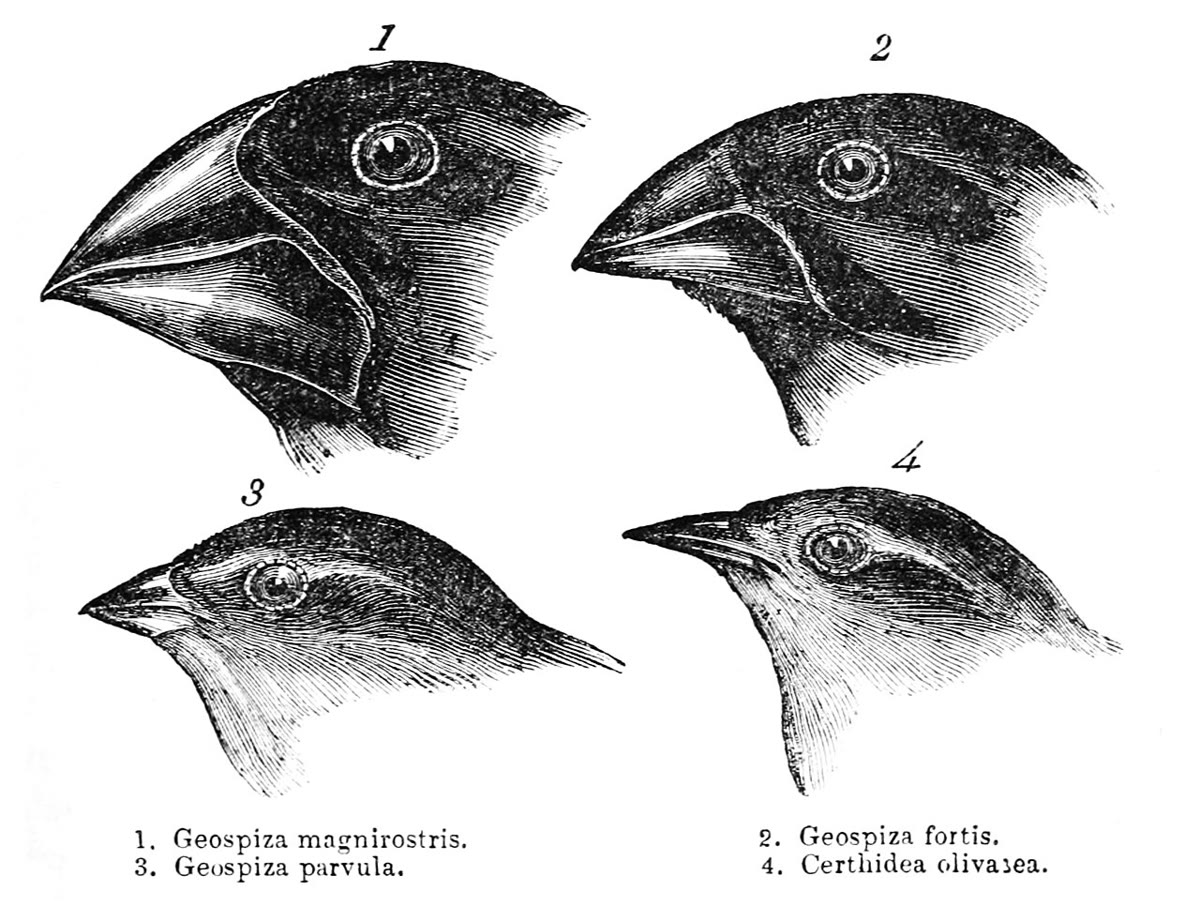
\includegraphics[width=0.62\linewidth]{images/book2/finches-gould.jpg}

{\small Vier vinken van Darwin, in 1845 door John Gould getekend naar de exemplaren die de \emph{Beagle} meebracht: in elk ander opzicht dezelfde vogel, met snavels van een notenkraker tot een naald. Eén groeisignaal, in het embryo anders gedoseerd, scheidt hen. Gravure, publiek domein.}
\end{omfigure}

\section{Samenleven: symbiose}

\begin{definition}[Symbiose]\label{def:g12:diversification-of-life:symbiosis}
Een \emph{symbiose}\index{symbiose} is een blijvend, nauw verbond van twee
\omterm{def:g10:biodiversity-scales:species}{soorten} waar beide voordeel bij hebben. Een korstmos is een schimmel die
algencellen huisvest die haar door \omterm{def:g10:cell-metabolism:autotrophy}{fotosynthese} voeden, terwijl zij hun
beschutting en water geeft; een koraal is een dier dat algen in zijn
weefsels huisvest; de wortels van de meeste planten zijn omhuld door
schimmels die mineralen leveren in ruil voor suiker; de darmen van dieren
bevatten bacteriën die verteren wat het dier niet kan. Het verbond brengt
organismen, structuren en levenswijzen voort die geen van beide partners
alleen zou kunnen bereiken.
\end{definition}

\begin{omfigure}
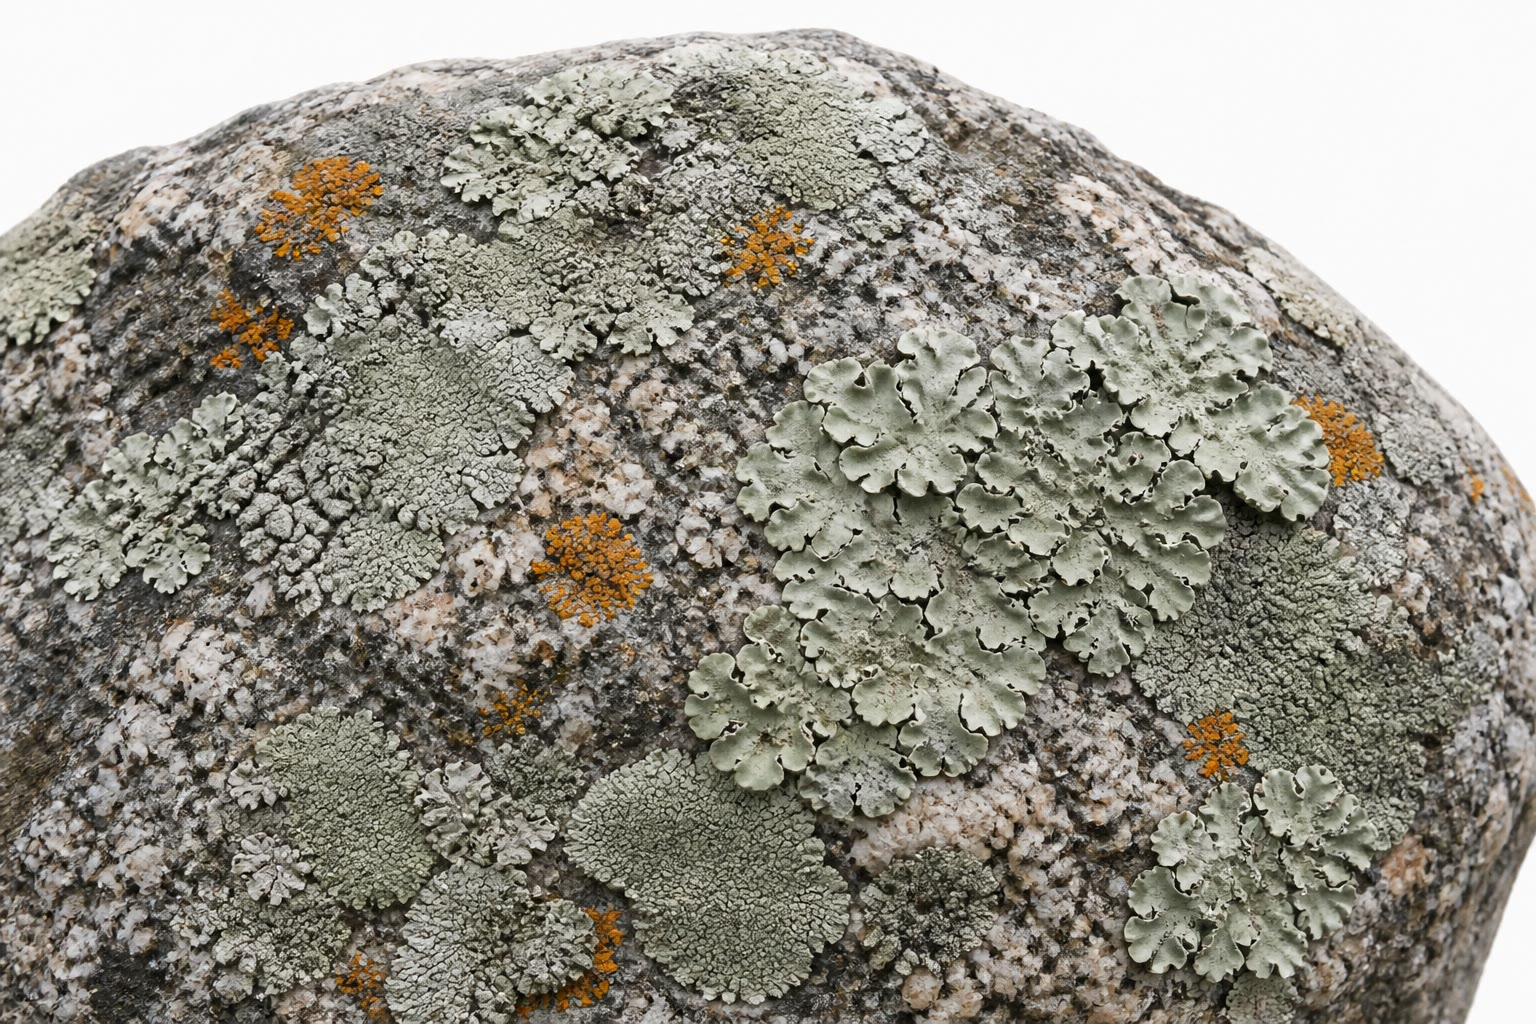
\includegraphics[width=0.58\linewidth]{images/book2/ai/g12-diversif-lichen.jpg}

{\small Korstmossen op een granieten zwerfkei. Elke plek is een schimmel en
een alg die tot één lichaam zijn uitgegroeid: een levensvorm die kaal
gesteente kan koloniseren en die geen van beide partners alleen aankan.}
\end{omfigure}

\begin{proposition}[De symbiose binnen in elke cel]\label{prop:g12:diversification-of-life:endosymbiosis}
De \omterm{def:g10:cells-common-unit:organelle}{mitochondriën} van elke \omterm{def:g10:cells-common-unit:prokaryote}{eukaryote cel}, en de \omterm{def:g10:cells-common-unit:organelle}{bladgroenkorrels} van
plantencellen, stammen af van vrij levende bacteriën die zo'n twee miljard
jaar geleden door een voorouderlijke \omterm{def:g10:cells-common-unit:cell}{cel} zijn opgeslokt en zijn gebleven.
De \omterm{def:g10:cells-common-unit:prokaryote}{eukaryote cel} zelf is de uitkomst van een \omterm{def:g12:diversification-of-life:symbiosis}{symbiose}.
\end{proposition}
\begin{proof}[Bewijsmateriaal]
\omterm{def:g10:cells-common-unit:organelle}{Mitochondriën} en \omterm{def:g10:cells-common-unit:organelle}{bladgroenkorrels} hebben hun eigen \omterm{def:g10:universal-dna:information}{DNA}, een klein ringetje
zoals dat van een bacterie, en hun eigen \omterm{def:g10:cells-common-unit:organelle}{ribosomen}, van het bacteriële
\omterm{def:g10:biodiversity-scales:species}{soort}, gevoelig voor de \omterm{def:g11:antibiotic-resistance:antibiotic}{antibiotica} die bacteriële maar geen eukaryote
\omterm{def:g10:cells-common-unit:organelle}{ribosomen} blokkeren; zij vermenigvuldigen zich door in tweeën te delen en
kunnen door de \omterm{def:g10:cells-common-unit:cell}{cel} niet opnieuw worden gemaakt; zij zijn in twee
membranen gewikkeld, waarvan het binnenste op een bacteriemembraan lijkt;
en hun \omterm{def:g10:universal-dna:gene}{genen} liggen in volgorde het dichtst bij die van bepaalde groepen
levende bacteriën --- purperbacteriën voor de \omterm{def:g10:cells-common-unit:organelle}{mitochondriën},
cyanobacteriën voor de \omterm{def:g10:cells-common-unit:organelle}{bladgroenkorrels}.
\end{proof}

\begin{omfigure}
\begin{tikzpicture}[font=\small, >=Stealth]
  % step 1: large cell + bacterium
  \draw[thick, fill=omDef!8] (0,0) ellipse (1.5 and 1.1);
  \draw[thick, fill=omDef!25] (-0.2,0.1) circle (0.4);
  \draw[thick, fill=omProp!40, rounded corners=4pt] (2.1,-0.15) rectangle (2.9,0.15);
  \node[anchor=north, align=center] at (0,-1.3) {voorouderlijke cel\\ met een celkern};
  \node[anchor=north, align=center] at (2.5,-0.4) {ademende\\ bacterie};
  \draw[->, thick] (3.6,0) -- (4.6,0) node[midway, above, font=\scriptsize] {opgeslokt};
  % step 2: bacterium inside
  \begin{scope}[xshift=6.3cm]
    \draw[thick, fill=omDef!8] (0,0) ellipse (1.5 and 1.1);
    \draw[thick, fill=omDef!25] (-0.4,0.15) circle (0.4);
    \draw[thick, fill=omProp!40, rounded corners=4pt] (0.35,-0.5) rectangle (1.15,-0.2);
    \node[anchor=north, align=center] at (0,-1.3) {behouden, niet verteerd;\\ deelt zich binnenin};
  \end{scope}
  \draw[->, thick] (8.2,0) -- (9.2,0) node[midway, above, font=\scriptsize, align=center] {twee miljard\\ jaar};
  % step 3: modern cell with mitochondria
  \begin{scope}[xshift=10.9cm]
    \draw[thick, fill=omDef!8] (0,0) ellipse (1.5 and 1.1);
    \draw[thick, fill=omDef!25] (-0.4,0.15) circle (0.4);
    \foreach \x/\y/\r in {0.5/0.4/20, 0.7/-0.3/-40, -0.2/-0.6/70}
      \draw[thick, fill=omProp!40, rotate around={\r:(\x,\y)}] (\x,\y) ellipse (0.3 and 0.13);
    \node[anchor=north, align=center] at (0,-1.3) {eukaryote cel:\\ mitochondriën};
  \end{scope}
\end{tikzpicture}

{\small De oorsprong van de \omterm{def:g10:cells-common-unit:organelle}{mitochondriën}. Een bacterie die door een
voorouderlijke \omterm{def:g10:cells-common-unit:cell}{cel} werd opgeslokt, bleef behouden en vermenigvuldigde zich
erbinnen; haar nakomelingen zijn de \omterm{def:g10:cells-common-unit:organelle}{mitochondriën} van elke eukaryoot, die
nog altijd hun eigen bacteriële \omterm{def:g10:universal-dna:information}{DNA} en \omterm{def:g10:cells-common-unit:organelle}{ribosomen} dragen. \omterm{def:g10:cells-common-unit:organelle}{Bladgroenkorrels}
zijn op dezelfde manier uit een fotosynthetische bacterie ontstaan.}
\end{omfigure}

\section{Verscheidenheid zonder genen: gedrag}

\begin{proposition}[Doorgegeven gedrag]\label{prop:g12:diversification-of-life:behaviour}
Bij veel dieren wordt een deel van wat een individu doet van anderen
geleerd --- door nabootsing, onderricht of nadoen --- en op zijn beurt
doorgegeven: een \emph{cultuur}\index{cultuur (dier)}, die zonder \omterm{def:g10:universal-dna:gene}{genen}
wordt overgedragen. Populaties van dezelfde \omterm{def:g10:biodiversity-scales:species}{soort} kunnen dus in gedrag
verschillen zoals zij in \omterm{def:g10:universal-dna:gene}{allelen} verschillen, en een gedrag kan zich in
één generatie door een populatie verbreiden in plaats van in de vele die
een \omterm{def:g11:mutations:mutation}{mutatie} nodig zou hebben.
\end{proposition}
\begin{proof}[Bewijsmateriaal]
Chimpanseegemeenschappen in verschillende bossen gebruiken verschillend
gereedschap --- hier stenen om noten te kraken, daar stokjes om termieten
mee te vissen, elders bladeren als sponzen --- en die verschillen volgen
niet de genetische verwantschap of de beschikbaarheid van materiaal; een
jonge chimpansee eigent zich de verzameling van zijn gemeenschap toe door
naar zijn ouderen te kijken. Zangvogels die in afzondering worden
grootgebracht, zingen een ruw lied; horen zij volwassen vogels, dan zingen
zij het plaatselijke dialect, dat over een verspreidingsgebied verandert
als een menselijk accent. Een troep makaken op een eiland leerde binnen
tien jaar van één jong vrouwtje zoete aardappelen in zee te wassen, en haar
nakomelingen doen het nog steeds.
\end{proof}

\begin{omfigure}
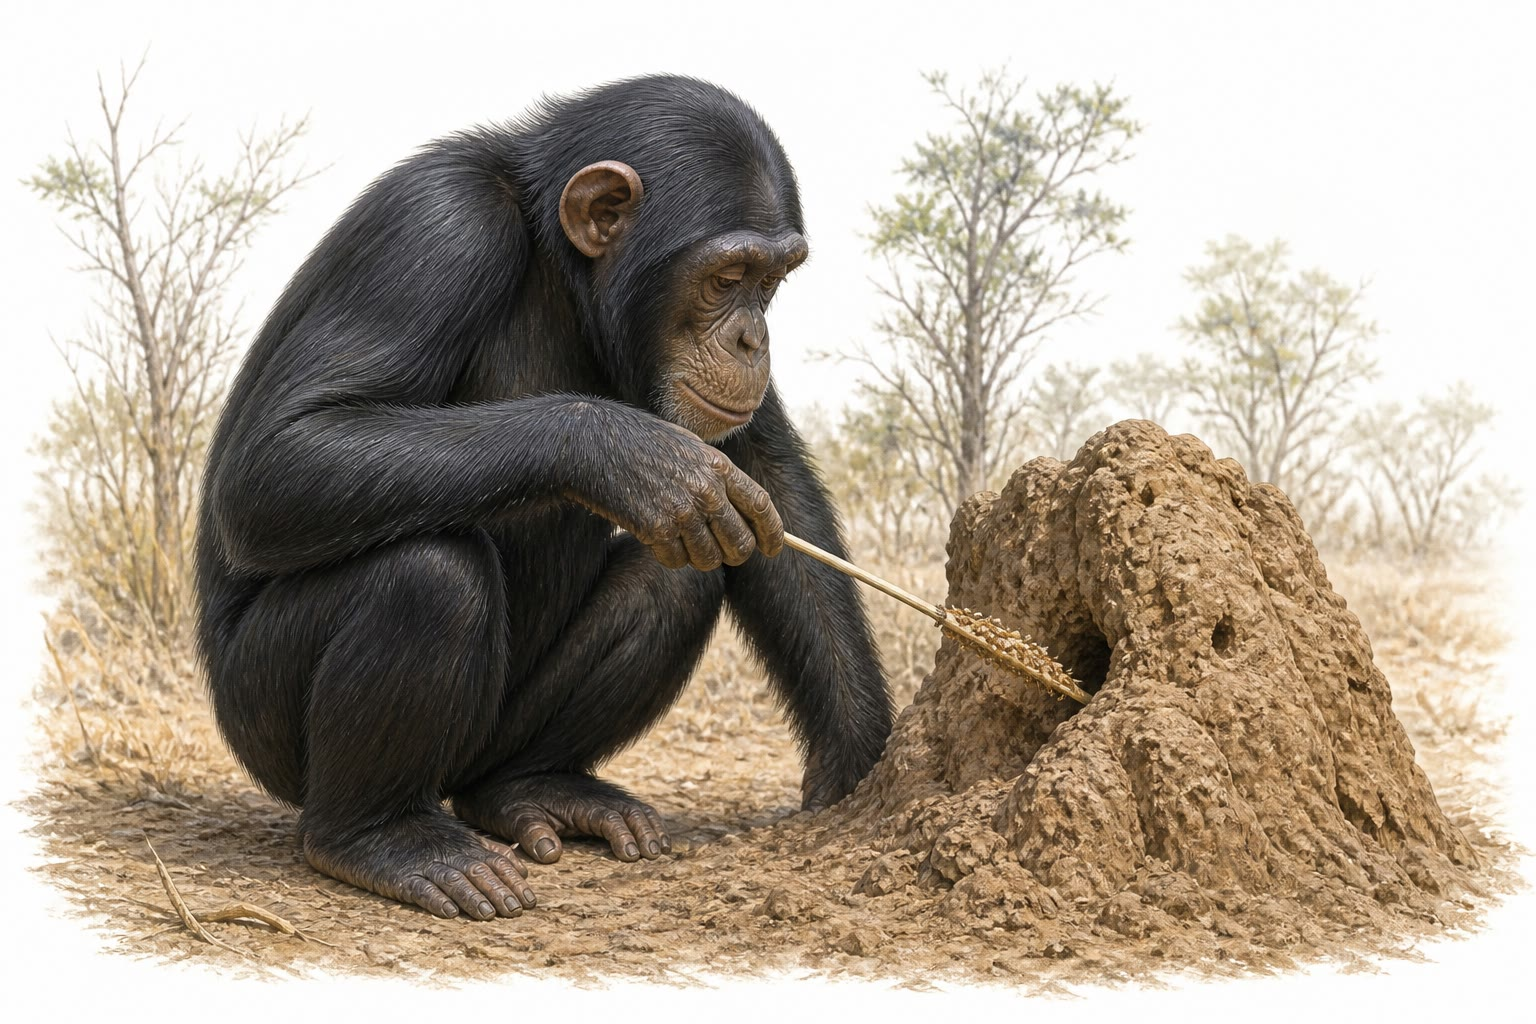
\includegraphics[width=0.6\linewidth]{images/book2/ai/g12-diversif-chimp-tool.jpg}

{\small Een chimpansee die met een toebereid stokje naar termieten vist.
De techniek wordt door kijken geleerd en verschilt van gemeenschap tot
gemeenschap: een traditie, zonder \omterm{def:g10:universal-dna:gene}{genen} doorgegeven.}
\end{omfigure}

\begin{method}[De bron van een verschil benoemen]\label{met:g12:diversification-of-life:name}
Sta je voor een verschil tussen twee organismen of populaties:
\begin{enumerate}
  \item Zit het in de volgorde van een \omterm{def:g10:universal-dna:gene}{gen} (\omterm{def:g11:mutations:mutation}{mutatie}, \omterm{def:g10:universal-dna:gene}{allel})? In het
        aantal kopieën van een \omterm{def:g10:universal-dna:gene}{gen} (verdubbeling)? In de aanwezigheid van
        een \omterm{def:g10:universal-dna:gene}{gen} van elders (horizontale overdracht)? In het aantal sets
        \omterm{def:g10:universal-dna:information}{chromosomen} (polyploïdie)?
  \item Zit het in wanneer, waar of hoe sterk een gedeeld \omterm{def:g10:universal-dna:gene}{gen} tijdens de
        ontwikkeling tot uiting komt (regeling)?
  \item Is het het gevolg van een verbond met een andere \omterm{def:g10:biodiversity-scales:species}{soort}
        (\omterm{def:g12:diversification-of-life:symbiosis}{symbiose})?
  \item Is het geleerd (gedrag dat door cultuur wordt doorgegeven) ---
        wel geërfd, maar niet genetisch?
\end{enumerate}
Vaak is er meer dan één antwoord juist; de vragen vormen de inventaris van
dit hoofdstuk.
\end{method}

\begin{remark}[Opsplitsing en selectie]\label{rem:g12:diversification-of-life:selection}
Elk proces hier brengt variatie voort; geen ervan beslist wat overleeft.
Een \omterm{prop:g12:diversification-of-life:polyploidy}{polyploïde} tarwe, het expressiepatroon van een python, een korstmos,
een traditie van notenkraken --- elk bleef bestaan omdat het werkte waar
het ontstond. Het sorteren van de variatie --- selectie, en toeval --- is
het onderwerp van het volgende hoofdstuk; dit hoofdstuk heeft uiteengezet
hoeveel er te sorteren valt, en op hoeveel manieren het wordt gemaakt.
\end{remark}

\section{Oefeningen}

\begin{exercise}[$\star$]\label{exo:g12:diversification-of-life:1}
Noem vijf bronnen van opsplitsing naast de puntmutatie.
\end{exercise}

\begin{exercise}[$\star$]\label{exo:g12:diversification-of-life:2}
Wat is een \omterm{prop:g12:diversification-of-life:duplication}{genfamilie}, en hoe ontstaat er een?
\end{exercise}

\begin{exercise}[$\star$]\label{exo:g12:diversification-of-life:3}
Waarom is een kruising tussen twee \omterm{def:g10:biodiversity-scales:species}{soorten} meestal onvruchtbaar, en hoe
kan chromosoomverdubbeling haar vruchtbaar maken?
\end{exercise}

\begin{exercise}[$\star$]\label{exo:g12:diversification-of-life:4}
Geef drie lijnen van bewijs dat \omterm{def:g10:cells-common-unit:organelle}{mitochondriën} van bacteriën afstammen.
\end{exercise}

\begin{exercise}[$\star$]\label{exo:g12:diversification-of-life:5}
Wat wordt met een cultuur bij dieren bedoeld? Geef een voorbeeld.
\end{exercise}

\begin{exercise}[$\star\star$]\label{exo:g12:diversification-of-life:6}
Emmertarwe heeft $2n = 28$ en eenkoorn $2n = 14$. Hoeveel \omterm{def:g10:universal-dna:information}{chromosomen}
heeft hun kruising, en hoeveel paren kunnen er bij haar \omterm{def:g12:meiosis-genetic-shuffling:meiosis}{meiose} worden
gevormd? Verklaar haar onvruchtbaarheid.
\end{exercise}

\begin{exercise}[$\star\star$]\label{exo:g12:diversification-of-life:7}
De \omterm{def:g10:universal-dna:gene}{genen} voor $\alpha$- en $\beta$-globine zijn voor 50\% gelijk; die voor
$\beta$ en $\gamma$ voor 80\%. Welke verdubbeling is ouder? Teken de boom.
\end{exercise}

\begin{exercise}[$\star\star$]\label{exo:g12:diversification-of-life:8}
Leg uit hoe een python geen poten kan hebben, terwijl hij de \omterm{def:g10:universal-dna:gene}{genen} draagt
die bij een hagedis poten bouwen.
\end{exercise}

\begin{exercise}[$\star\star$]\label{exo:g12:diversification-of-life:9}
Twee vinkensoorten verschillen een factor twee in snaveldiepte maar hebben
dezelfde snavelgenen. Waar zit het verschil, en waarom kan het snel
ontstaan?
\end{exercise}

\begin{exercise}[$\star\star$]\label{exo:g12:diversification-of-life:10}
Een korstmos dat uit alleen zijn schimmel wordt gekweekt, is een vormeloze
schimmelmassa; uit alleen zijn alg een groen vlies. Leg uit in welke zin
het korstmos een nieuw \omterm{def:g10:biodiversity-scales:species}{soort} organisme is.
\end{exercise}

\begin{exercise}[$\star\star$]\label{exo:g12:diversification-of-life:11}
Een populatie chimpansees kraakt noten; een naburige populatie aan de
overkant van een rivier niet, hoewel er aan beide kanten noten en stenen
in overvloed zijn. Bepaal met \cref{met:g12:diversification-of-life:name}
de bron van het verschil en verantwoord dat.
\end{exercise}

\begin{exercise}[$\star\star\star$]\label{exo:g12:diversification-of-life:12}
Een \omterm{def:g10:universal-dna:gene}{gen} van het menselijke genoom is vrijwel gelijk aan een \omterm{def:g10:universal-dna:gene}{gen} van een
virus en aan niets in enig ander zoogdier behalve de primaten. Stel een
geschiedenis ervoor voor, en zeg hoe je die zou toetsen.
\end{exercise}

\begin{exercise}[$\star\star\star$]\label{exo:g12:diversification-of-life:13}
\omterm{def:g11:antibiotic-resistance:antibiotic}{Antibiotica} die bacteriële \omterm{def:g10:cells-common-unit:organelle}{ribosomen} blokkeren, hebben bij hoge doses
bijwerkingen op de \omterm{def:g10:cells-common-unit:organelle}{mitochondriën} van de patiënt. Leg uit waarom, en wat
dat zegt over de afstamming van de \omterm{def:g10:cells-common-unit:organelle}{mitochondriën}.
\end{exercise}

\begin{exercise}[$\star\star\star$]\label{exo:g12:diversification-of-life:14}
Leg uit waarom een nieuwe \omterm{prop:g12:diversification-of-life:polyploidy}{polyploïde} \omterm{def:g10:biodiversity-scales:species}{soort} vanaf de eerste generatie van
haar ouders is afgezonderd, terwijl een nieuw \omterm{def:g10:universal-dna:gene}{allel} vele generaties nodig
heeft om zich te verbreiden. Wat betekent dat voor de snelheid waarmee
plantensoorten kunnen ontstaan?
\end{exercise}

\begin{exercise}[$\star\star\star$]\label{exo:g12:diversification-of-life:15}
"Alle verscheidenheid komt van \omterm{def:g11:mutations:mutation}{mutatie}." Bespreek dit in een alinea: in
welke zin die uitspraak in de grond waar is, en in welke opzichten de
processen van dit hoofdstuk verder gaan.
\end{exercise}

\section{Probleem: Drie grassen in een brood}

\begin{problem}[{Weekendprobleem --- de geschiedenis van broodtarwe uit
chromosomen gereconstrueerd, de genen van een python naast die van een
muis gelezen, en de bacterie in elke cel voor het gerecht gebracht}]
\label{pb:g12:diversification-of-life:1}
Eenkoorn (AA), geitengras 1 (BB) en geitengras 2 (DD) hebben elk
$2n = 14$. Emmer is AABB en broodtarwe AABBDD.

\medskip
\noindent\textbf{Deel I --- De \omterm{def:g10:universal-dna:information}{chromosomen} van de tarwe.}
\begin{enumerate}
  \item Geef het aantal \omterm{def:g10:universal-dna:information}{chromosomen} in emmer en in broodtarwe.
  \item De kruising van eenkoorn en geitengras 1 heeft 14 \omterm{def:g10:universal-dna:information}{chromosomen}, 7
        van elke \omterm{def:g10:biodiversity-scales:species}{soort}. Hoeveel paren homologen vormen zich bij haar
        \omterm{def:g12:meiosis-genetic-shuffling:meiosis}{meiose}? Hoe zien haar gameten eruit?
  \item Leg uit waarom een verdubbeling van haar \omterm{def:g10:universal-dna:information}{chromosomen} de
        vruchtbaarheid herstelt: tel de paren.
  \item De kruising van emmer en geitengras 2 heeft 21 \omterm{def:g10:universal-dna:information}{chromosomen}. Welke
        daarvan kunnen paren, en waarom is zij onvruchtbaar?
  \item Na verdubbeling heeft broodtarwe er 42. Hoeveel paren vormen zich
        bij haar \omterm{def:g12:meiosis-genetic-shuffling:meiosis}{meiose}, en hoeveel \omterm{def:g10:universal-dna:information}{chromosomen} draagt een stuifmeelkorrel?
\end{enumerate}

\medskip
\noindent\textbf{Deel II --- De geschiedenis lezen.}
\begin{enumerate}[resume]
  \item Broodtarwe draagt van de meeste \omterm{def:g10:universal-dna:gene}{genen} drie kopieën, één op elke
        set. Leg uit waarom een \omterm{def:g11:mutations:mutation}{mutatie} die één kopie onbruikbaar maakt
        meestal geen zichtbaar gevolg heeft, en wat dat op den duur
        mogelijk maakt.
  \item Emmer werd 10\,000 jaar geleden verbouwd en broodtarwe duikt
        8\,000 jaar geleden in vindplaatsen op. Waar en wanneer vond de
        tweede kruising waarschijnlijk plaats? Wat moest er naast elkaar
        groeien?
  \item Kruisingen van emmer met geitengras 2 in het laboratorium,
        gevolgd door chemische verdubbeling, geven vruchtbare planten die
        op broodtarwe lijken. Welke conclusie uit die geschiedenis
        bevestigt dat?
  \item Broodtarwe kan zich niet met eenkoorn kruisen tot vruchtbare
        nakomelingen. Is zij een aparte \omterm{def:g10:biodiversity-scales:species}{soort}? Verantwoord dat met de
        definitie uit \cref{ch:g10:biodiversity-scales}.
  \item Een veredelaar wil een \omterm{def:g10:universal-dna:gene}{gen} voor ziekteweerstand uit geitengras 2
        in broodtarwe inbrengen. Leg uit waarom dat gemakkelijker is dan
        vanuit een niet-verwante plant.
\end{enumerate}

\medskip
\noindent\textbf{Deel III --- De \omterm{def:g10:universal-dna:gene}{genen} van de python.}
\begin{enumerate}[resume]
  \item De gebiedsgenen van de romp zijn tussen muis en python voor 98\%
        gelijk. Wat zegt dat over de bron van het verschil in hun
        lichamen?
  \item In het muizenembryo is het \omterm{def:g10:universal-dna:gene}{gen} voor "romp met ribben" over 13
        segmenten actief; bij de python over ongeveer 300. Benoem het
        \omterm{def:g10:biodiversity-scales:species}{soort} verandering waar het om gaat.
  \item Het pythonembryo vormt kleine knopjes waar achterpoten zouden
        komen, die daarna ophouden te groeien. Wat suggereert dat over de
        pootgenen en over het signaal dat hen zou aanzetten?
  \item Muizen die zo zijn veranderd dat zij het \omterm{def:g10:universal-dna:gene}{gen} voor "romp met
        ribben" ook in het lendengebied tot uiting brengen, krijgen daar
        extra ribben. Wat voegt die proef aan de vergelijking toe?
  \item Vergelijk de twee typen verandering: die van broodtarwe en die
        van de python. Welke veranderde de omvang van het genoom, en
        welke het gebruik ervan?
\end{enumerate}

\medskip
\noindent\textbf{Deel IV --- De bacterie binnenin.}
\begin{enumerate}[resume]
  \item Noem vier kenmerken van \omterm{def:g10:cells-common-unit:organelle}{mitochondriën} die bij een bacteriële
        oorsprong passen, en zeg voor elk wat je zou verwachten als de
        \omterm{def:g10:cells-common-unit:cell}{cel} de \omterm{def:g10:cells-common-unit:organelle}{mitochondriën} in plaats daarvan van de grond af had
        gebouwd.
  \item Het \omterm{def:g10:universal-dna:information}{DNA} van de \omterm{def:g10:cells-common-unit:organelle}{mitochondriën} draagt maar 37 \omterm{def:g10:universal-dna:gene}{genen}, terwijl het
        \omterm{def:g10:cells-common-unit:organelle}{mitochondrion} ongeveer 1500 \omterm{def:g10:chemistry-of-life:families}{eiwitten} nodig heeft. Waar zijn de
        andere \omterm{def:g10:universal-dna:gene}{genen}, en wat is er in twee miljard jaar met hen gebeurd?
  \item Elk \omterm{def:g10:cells-common-unit:organelle}{mitochondrion} van een mens komt uit de eicel, geen enkel uit
        de zaadcel. Wat volgt daaruit voor de overerving van
        mitochondriale \omterm{def:g10:universal-dna:gene}{genen}, en voor het volgen van de moederlijke
        afstamming?
  \item Een korstmos en een \omterm{def:g10:cells-common-unit:organelle}{mitochondrion} zijn allebei \omterm{def:g12:diversification-of-life:symbiosis}{symbiosen}. In welk
        opzicht is die van het \omterm{def:g10:cells-common-unit:organelle}{mitochondrion} verder gegaan?
  \item Geef het resultaat: de drie \omterm{def:g10:biodiversity-scales:species}{soorten} in een brood en het aantal
        \omterm{def:g10:universal-dna:information}{chromosomen} dat elk bijdroeg; het ene woord dat benoemt wat er
        verschilt tussen het gebruik dat de python en de muis van hun
        gedeelde \omterm{def:g10:universal-dna:gene}{genen} maken; en het \omterm{def:g10:cells-common-unit:organelle}{organel} dat een voormalige bacterie
        is.
\end{enumerate}
\end{problem}
